%\documentclass[handout]{beamer}
\documentclass{beamer}

\mode<presentation>
{
\usetheme{default}
\usefonttheme[onlymath]{serif}
%\usetheme{Singapore}
%\usetheme{Warsaw}
%\usetheme{Malmoe}
% \useinnertheme{circles}
% \useoutertheme{infolines}
% \useinnertheme{rounded}

\setbeamercovered{transparent=5}
}

\usepackage[english]{babel}
\usepackage[latin1]{inputenc}
\usepackage{textpos,alltt,listings,multirow,ulem,siunitx}
\newcommand\hmmax{0}
\newcommand\bmmax{0}
\usepackage{bm}

% font definitions, try \usepackage{ae} instead of the following
% three lines if you don't like this look
\usepackage{mathptmx}
\usepackage[scaled=.90]{helvet}
%\usepackage{courier}
\usepackage[T1]{fontenc}
\usepackage{tikz}
\usetikzlibrary[shapes,shapes.arrows,arrows,shapes.misc,fit,positioning]

% \usepackage{pgfpages}
% \pgfpagesuselayout{4 on 1}[a4paper,landscape,border shrink=5mm]

\usepackage{slashbox,multirow,listings,booktabs}
\usepackage{xspace}
\makeatletter
\DeclareRobustCommand\onedot{\futurelet\@let@token\@onedot}
\def\@onedot{\ifx\@let@token.\else.\null\fi\xspace}
\def\eg{{e.g}\onedot} \def\Eg{{E.g}\onedot}
\def\ie{{i.e}\onedot} \def\Ie{{I.e}\onedot}
\def\cf{{c.f}\onedot} \def\Cf{{C.f}\onedot}
\def\etc{{etc}\onedot}
\def\vs{{vs}\onedot}
\def\wrt{w.r.t\onedot}
\def\dof{d.o.f\onedot}
\def\etal{{et al}\onedot}
\makeatother

\usepackage{tikz}
\usetikzlibrary[shapes,shapes.arrows,arrows,shapes.misc,fit,positioning]

\usepackage{siunitx}
\DeclareSIUnit\year{a}
\DeclareSIUnit\byte{B}
\sisetup{retain-unity-mantissa = false}

\usepackage{fancyvrb}
\usepackage{minted}
\newminted{c}{gobble=2}
\newminted{python}{gobble=2}
%\newmint[cverb]{c}{} 
\newcommand\cverb[1][]{\SaveVerb[%
    aftersave={\textnormal{\UseVerb[#1]{vsave}}}]{vsave}}
\newcommand\cfunc[1][]{\SaveVerb[%
    aftersave={\textnormal{\UseVerb[#1]{vsave}\texttt{()}}}]{vsave}}
\newcommand\pyverb[1][]{\SaveVerb[%
    aftersave={\textnormal{\UseVerb[#1]{vsave}}}]{vsave}}
\def\asm#1{{\tt #1}}
\def\code#1{{\tt #1}}
\def\shell#1{{\tt \$ #1}}

\newcommand\email[1]{{\href{mailto:#1}{\nolinkurl{#1}}}}

\newcommand{\II}{\mathcal{I}}
\newcommand{\C}{\mathbb{C}}
\newcommand{\D}{\mathcal{D}}
\newcommand{\EE}{\mathcal{E}}
\newcommand{\F}{\mathcal{F}}
\newcommand{\I}{\mathcal{I}}
\newcommand{\N}{\mathcal{N}}
\newcommand{\PP}{\mathcal{P}}
\newcommand\Ppc{\ensuremath{\mathsf P}}
\newcommand{\bigO}{\ensuremath{\mathcal{O}}}
\newcommand{\R}{\mathbb{R}}
\newcommand{\Rz}{\mathcal{R}}
\newcommand{\QQ}{\mathcal Q}
\newcommand{\VV}{\mathcal V}
\newcommand{\ASM}{\mathrm{ASM}}
\newcommand{\RASM}{\mathrm{RASM}}

\newcommand{\kb}{\tt}
\newcommand{\Pk}[1]{\ensuremath{P_{#1}}}
\newcommand{\Qk}[1]{\ensuremath{Q_{#1}}}
\newcommand{\Pkdisc}[1]{\ensuremath{P_{#1}^{\text{disc}}}}
\newcommand{\Qkdisc}[1]{\ensuremath{Q_{#1}^{\text{disc}}}}
\newcommand{\blue}{\textcolor{blue}}
\newcommand{\green}{\textcolor{green!70!black}}
\newcommand{\red}{\textcolor{red}}
\newcommand{\brown}{\textcolor{brown}}
\newcommand{\cyan}{\textcolor{cyan}}
\newcommand{\magenta}{\textcolor{magenta}}
\newcommand{\yellow}{\textcolor{yellow}}
\newcommand{\mini}{\mathop{\rm minimize}}
\newcommand{\st}{\mbox{subject to }}
\newcommand{\lap}{\Delta}
\newcommand{\grad}{\nabla}
\newcommand\mtab{\hspace{\stretch{1}}}
\newcommand\ud{\,\mathrm{d}}
\newcommand\bslash{{$\backslash$}}
\newcommand\half{{\frac 1 2}}
\newcommand{\abs}[1]{\left\lvert #1 \right\rvert}
\newcommand{\bigabs}[1]{\big\lvert #1 \big\rvert}
\newcommand{\norm}[1]{\left\lVert #1 \right\rVert}
\newcommand\oneitem[1]{\begin{itemize} \item #1 \end{itemize}}
\newcommand\pfrak{{\mathfrak p}}
\newcommand\nfrak{{\mathfrak n}}
\newcommand\ff{\bm f}
\newcommand\mm{\bm m}
\newcommand\nn{\bm n}
\newcommand\uu{\bm u}
\newcommand\vv{\bm v}
\newcommand\ww{\bm w}
\newcommand\DD{D}
\newcommand{\tcolon}{\!:\!}
\DeclareMathOperator{\sgn}{sgn}
\DeclareMathOperator{\card}{card}
\DeclareMathOperator{\trace}{tr}
\DeclareMathOperator{\erf}{erf}
\DeclareMathOperator{\sspan}{span}
\renewcommand{\bar}{\overline}
% \DeclareMathOperator{\divergence}{div}
% \renewcommand\div\divergence
\renewcommand{\div}{{\nabla \cdot}}
\newcommand\spliceop{\leftrightsquigarrow}
\newcommand\splice[5]{{#1} \overset{#5}{\underset{#3,#4}{\leftrightsquigarrow}} {#2}}
\newcommand{\ip}[2]{{\left\langle #1, #2 \right\rangle}}
\newcommand{\Linfty}{{L^\infty}}

% Dimensionless numbers
\newcommand{\Peclet}{{\mathrm{Pe}}}
\newcommand{\Reynolds}{{\mathrm{Re}}}
\newcommand{\Rayleigh}{{\mathrm{Ra}}}
\newcommand{\Mach}{{\mathrm{Ma}}}
\newcommand{\Prandtl}{{\mathrm{Pr}}}
\newcommand{\Grashof}{{\mathrm{Gr}}}

\newcommand{\PETSc}{{PETSc}}
\newcommand{\Dohp}{{Dohp}}
\newcommand\libmesh{\texttt{libMesh}}
\newcommand\dealii{\texttt{Deal.II}}
\newcommand\MatMult{\cverb|MatMult|}
\newcommand\MatSolve{\cverb|MatSolve|}
\newcommand{\secref}[1]{{Section~\ref{#1}}}
\newcommand{\chapref}[1]{{Chapter~\ref{#1}}}
\newcommand{\figref}[1]{{Figure~\ref{#1}}}
\newcommand{\tabref}[1]{{Table~\ref{#1}}}
\newcommand\AIJ{{\cverb|AIJ|}}
\newcommand\AIJInode{\cverb|AIJ|/\cverb|Inode|}
\newcommand\BAIJ[1][]{\ifthenelse{\equal{#1}{}}{\cverb|BAIJ|}{\ensuremath{\cverb|BAIJ|(#1)}}}
\newcommand\SBAIJ[1][]{\ifthenelse{\equal{#1}{}}{\cverb|SBAIJ|}{\ensuremath{\cverb|SBAIJ|(#1)}}}
\newcommand\todo[1]{{\color{red}\bf [TODO: #1]}}
\newcommand\tf[1]{\hat{#1}}     % test functions


\title{Implicit solution of free surface flows in glaciology}

\author{Jed Brown}


% - Use the \inst command only if there are several affiliations.
% - Keep it simple, no one is interested in your street address.
\institute[ETH Z\"urich]
{
  Laboratory of Hydrology, Hydraulics, and Glaciology \\
  ETH Z�rich
}

\date[2011-03-01]{2011-03-01}

% This is only inserted into the PDF information catalog. Can be left
% out.
\subject{Talks}


% If you have a file called "university-logo-filename.xxx", where xxx
% is a graphic format that can be processed by latex or pdflatex,
% resp., then you can add a logo as follows:

% \pgfdeclareimage[height=0.5cm]{university-logo}{university-logo-filename}
% \logo{\pgfuseimage{university-logo}}



% Delete this, if you do not want the table of contents to pop up at
% the beginning of each subsection:
% \AtBeginSubsection[]
% {
% \begin{frame}<beamer>
% \frametitle{Outline}
% \tableofcontents[currentsection,currentsubsection]
% \end{frame}
% }

% If you wish to uncover everything in a step-wise fashion, uncomment
% the following command:

%\beamerdefaultoverlayspecification{<+->}

\begin{document}
\lstset{language=C}
\normalem

\begin{frame}
\titlepage
\end{frame}

% \begin{frame}
%   \frametitle{Outline}
%   \tableofcontents
%   % You might wish to add the option [pausesections]
% \end{frame}

% \section{Practicalities}

\begin{frame}
  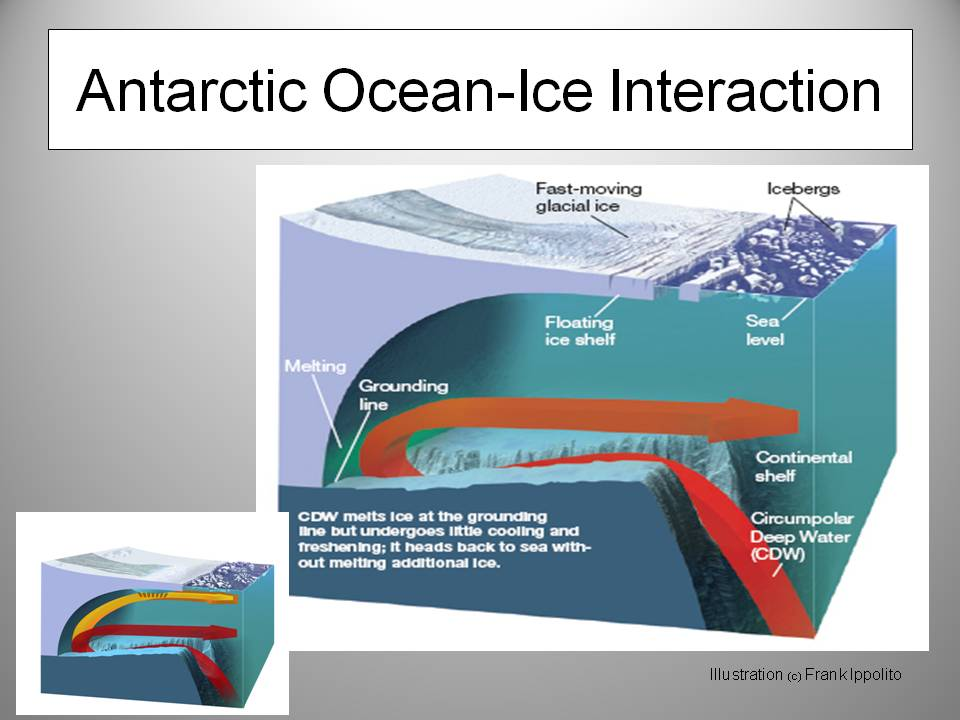
\includegraphics[width=\textwidth]{figures/GroundingLine/NaturalHistory2008} \\
  \vspace{-.5em}
  {\tiny Bindschadler 2008}
\end{frame}


\section[Hydrostatic]{A robust multigrid solver for the hydrostatic equations}
\begin{frame}[shrink=5]{Hydrostatic equations for ice sheet flow}
  \begin{itemize}
  \item Valid when $w_x \ll u_z$, independent of basal friction {\small (Schoof\&Hindmarsh 2010)}
  \item Eliminate $p$ and $w$ from Stokes by incompressibility:\\
    \quad 3D elliptic system for $\bm u = (u,v)$
    \begin{align*}
      - \nabla\cdot \left[ \eta
        \begin{pmatrix}
          4 u_x + 2 v_y & u_y + v_x & u_z \\
          u_y + v_x & 2 u_x + 4 v_y & v_z
        \end{pmatrix} \right] + \rho g \bar\nabla h & = 0
    \end{align*}
    \begin{align*}
      \eta(\theta,\gamma) &= \frac{B(\theta)}{2} (\gamma_0 + \gamma)^{\frac{1-\mathfrak n}{2\mathfrak n}}, \qquad \mathfrak n \approx 3 \\
      \gamma &= u_x^2 + v_y^2 + u_xv_y + \frac 1 4 (u_y+v_x)^2 + \frac 1 4 u_z^2 + \frac 1 4 v_z^2
    \end{align*}
    and slip boundary $\sigma \cdot \bm n = \beta^2 \bm u$ where
    \begin{align*}
      \beta^2(\gamma_b) &= \beta_0^2 (\epsilon_b^2 + \gamma_b)^{\frac{\mathfrak m-1}{2}}, \qquad 0 < \mathfrak m \le 1 \\
      \gamma_b &= \frac 1 2 (u^2 + v^2)
    \end{align*}
  \item $Q_1$ FEM with Newton-Krylov-Multigrid solver in PETSc: \code{src/snes/examples/tutorials/ex48.c}
  \end{itemize}
\end{frame}

\begin{frame}
  \includegraphics[width=\textwidth]{figures/THI/x-shear}
\end{frame}
\begin{frame}
  \includegraphics[width=\textwidth]{figures/THI/x-80km-m16p2l6-ew} \\
  Grid-sequenced Newton-Krylov solution of test $X$.  The solid lines denote nonlinear iterations, and the dotted lines with $\times$ denote linear residuals.
\end{frame}
\frame{
  \vspace{-1em}
  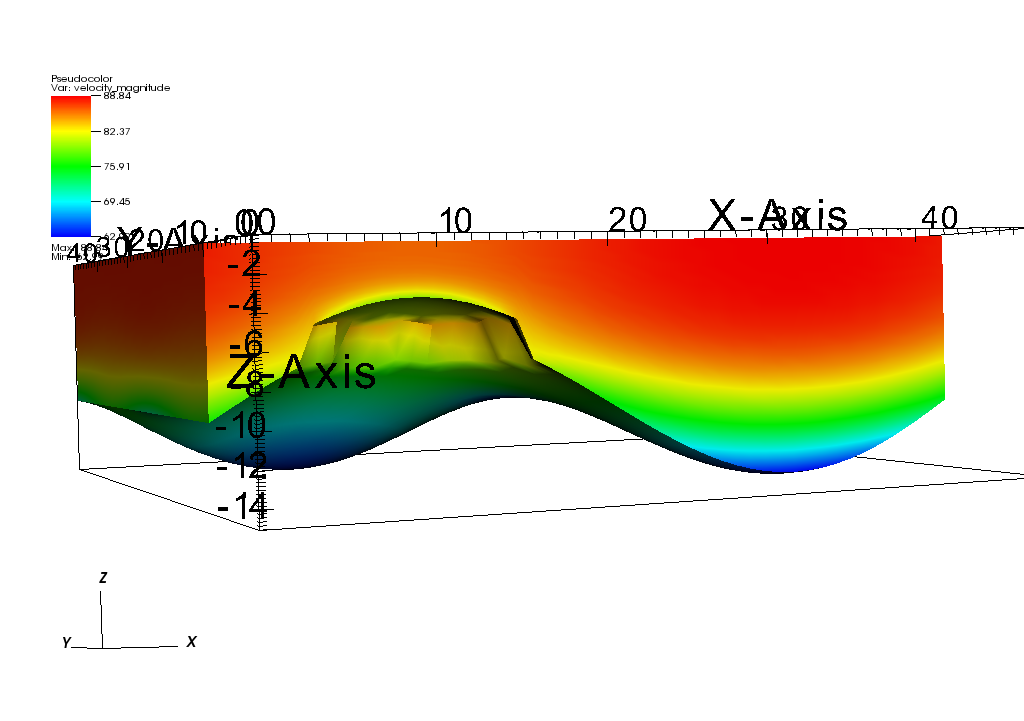
\includegraphics[width=\textwidth]{figures/THI/y-5km-m6p5l4-clip}
  \vspace{-3.5em}
  \begin{itemize}
  \item Bathymetry is essentially discontinuous on any grid
  \item Shallow ice approximation produces oscillatory solutions
  \item Nonlinear and linear solvers have major problems or fail
  \item Grid sequenced Newton-Krylov multigrid works \\
    as well as in the smooth case
  \end{itemize}
}

\begin{frame}
  \begin{figure}
    \includegraphics[width=\textwidth]{figures/THI/y-10km-m10p6l5-ew}
    \centering\caption{Grid sequenced Newton-Krylov convergence for test $Y$.
    The ``cliff'' has \SI{58}{\degree} angle in the red line ($12\times 125$ meter elements), \SI{73}{\degree} for the cyan line ($6\times 62$ meter elements).}\label{fig:testy}
  \end{figure}
\end{frame}
\begin{frame}
  \begin{figure}
    \includegraphics[width=\textwidth]{figures/THI/linear4}
    \centering\caption{Average number of Krylov iterations per nonlinear iteration.  Each nonlinear system was solved to a relative tolerance of $10^{-2}$.}\label{fig:linear}
  \end{figure}
\end{frame}

\begin{frame}{Strong scaling on Blue Gene/P (Shaheen)}
\begin{figure}
  \includegraphics[width=\textwidth]{figures/THI/shaheen-strong}
  \centering\caption{Strong scaling on Shaheen for different size coarse levels problems and different coarse level solvers.
    The straight lines on the strong scaling plot have slope $-1$ which is optimal.}\label{fig:shaheen-strong}
\end{figure}
\end{frame}

\begin{frame}{Weak scaling on Blue Gene/P (Shaheen)}
  \begin{figure}
  \includegraphics[width=\textwidth]{figures/THI/shaheen-weak}
  \centering\caption{Weak scaling on Shaheen with a breakdown of time spent in different phases of the solution process.
    Times are for the full grid-sequenced problem, not just the finest level solve.}\label{fig:shaheen-weak}
\end{figure}
\end{frame}

\begin{frame}
  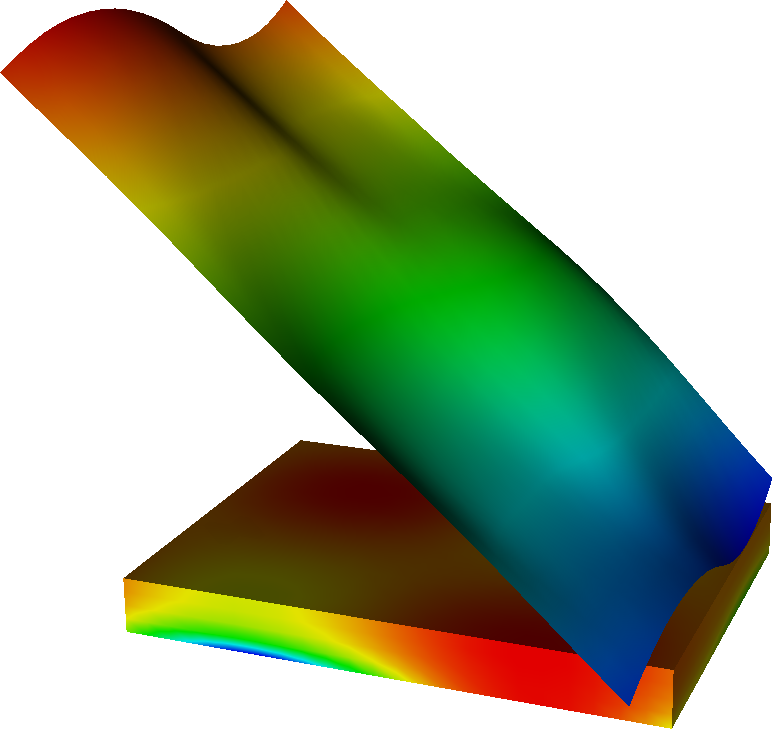
\includegraphics[width=0.8\textwidth]{figures/THI/c-steady-crop}
\end{frame}

% \section{Other models}
% \begin{frame}{Standard shallow approximations}
  \begin{itemize}
  \item Shallow Ice Approximation (SIA):
    \begin{itemize}
    \item Purely local definition of velocity
      \begin{align*}
        u(z) &= - (\rho g)^{\mathfrak n} \int_b^z A(T(z))
        (h-z)^{\mathfrak n} \abs{\bar\nabla h}^{\mathfrak n-1} \bar\nabla h
      \end{align*}
    \item No membrane stresses so only acceptable for \alert<2>{$\lambda \gg 1$}
    \item No solve so costs similar to one residual evaluation per time step
    \end{itemize}
  \item ``Shelfy Stream'' Approximation (SSA)
    \begin{itemize}
    \item Need to solve elliptic problem posed in the map plane (2D):
      \begin{gather*}
        -\bar\nabla\cdot \left[H \bar\eta
          \begin{pmatrix}
            4\bar u_x + 2\bar v_y & \bar v_x + \bar u_y \\
            \bar v_x + \bar u_y   & 2\bar u_x + 4\bar v_y
          \end{pmatrix} \right]
        + \beta^2 \bm{\bar u} + \rho g H \bar\grad h = 0 \\
        \eta(\theta,\gamma) = \frac{B(\theta)}{2} (\gamma_0 + \gamma)^{\frac{1-\mathfrak n}{2\mathfrak n}}, \qquad \mathfrak n \approx 3 \\
        \gamma = \bar u_x^2 + \bar v_y^2 + \bar u_x\bar v_y + \frac 1 4 (\bar u_y+\bar v_x)^2 %{\color{gray} + \frac 1 4 u_z^2 + \frac 1 4 v_z^2}
      \end{gather*}
    \item No vertical shear so only acceptable when \alert<2>{$\lambda \ll 1$}
    \end{itemize}
  \end{itemize}
\end{frame}

\begin{frame}{Vertically-integrated Hybrids}
  \begin{itemize}
  \item Daniel Goldberg 2010, same order of accuracy as hydrostatic
    \begin{itemize}
    \item Vertically average ``membrane'' part of hydrostatic equations
      \begin{gather*}
        -\bar\nabla\cdot \left[\bar\eta
          \begin{pmatrix}
            4\bar u_x + 2\bar v_y & \bar v_x + \bar u_y   \\
            \bar v_x + \bar u_y   & 2\bar u_x + 4\bar v_y
          \end{pmatrix} \right]
        {\color{red} - \left[ \eta \begin{pmatrix} u_z \\ v_z \end{pmatrix} \right]_z}
        + \beta^2 \bm{\bar u} + \rho g H \bar\grad h = 0 \\
        \eta(\theta,\gamma) = \frac{B(\theta)}{2} (\gamma_0 + \gamma)^{\frac{1-\mathfrak n}{2\mathfrak n}}, \qquad \mathfrak n \approx 3 \\
        \gamma = \bar u_x^2 + \bar v_y^2 + \bar u_x\bar v_y + \frac 1 4 (\bar u_y+\bar v_x)^2 {\color{red} + \frac 1 4 u_z^2 + \frac 1 4 v_z^2}
      \end{gather*}
    \item Solve by integrating $z$-dependence and $\eta$, solve linear elliptic problem in map plane for $\bm{\bar u}$, iterate (Picard, $\approx 50$ its)
    \item Evaluating viscosity (or a Newton residual) costs about \\ one hydrostatic residual
    \end{itemize}
  \item Bueler and Brown 2009, used in PISM
    \begin{itemize}
    \item Ad-hoc combination of independent SSA and SIA solutions
    \item Lower formal order of accuracy, but nonlinear solve is strictly 2D
    \end{itemize}
  \end{itemize}
\end{frame}

% \begin{frame}{Non-Newtonian Stokes system: velocity $\bm u$, pressure $p$}
% \begin{columns}
% \begin{column}{0.5\textwidth}
%   \alert{\begin{align*}
%     -\nabla \cdot(\eta D\uu) + \nabla p - \ff &= 0 \\
%     \nabla \cdot \uu &= 0
%   \end{align*}}
% \end{column}
% \begin{column}{0.5\textwidth}
%     \begin{align*}
%       D\uu &= \tfrac 1 2 \left(\nabla \uu + (\nabla \uu)^T \right) \\
%       \gamma(D\uu) &= \tfrac 1 2 D\uu \tcolon D\uu \\
%       \eta(\gamma) &= B(\theta,\dotsc)\big(\gamma_0 + \gamma \big)^{\frac{\mathfrak{p}-2}{2}} \\
%       \mathfrak{p} &= 1 + \tfrac{1}{\mathfrak{n}} \approx \tfrac 4 3 \\
%       T &= \bm 1 - \bm n \otimes \bm n \\
%     \end{align*}
% \end{column}
% \end{columns}
% \vspace{-1.5em}
%     with boundary conditions
%     \begin{align*}
%       (\eta D\bm u - p\bm 1)\cdot\bm n =
%       \begin{cases}\bm 0 & \text{free surface} \\
%         -\rho_w z \bm n & \text{ice-ocean interface}\end{cases} \\
%       \bm u = \bm 0\qquad\qquad \text{frozen bed}, \theta < \theta_0 \\
%       \left. \begin{aligned}
%           \bm u \cdot \bm n &= \bm g_{\text{melt}}(T\uu,\dotsc) \\
%           T (\eta D\bm u - p\bm 1)\cdot\bm n &= \bm g_{\text{slip}}(T \bm u,\dotsc) \end{aligned}\right\}
%       \text{nonlinear slip}, \theta \ge \theta_0 \\
%     \end{align*}
%     \vspace{-3em}
%     \[ \bm g_{\text{slip}}(T\uu) = \beta_{\mathfrak{m}}(\dotsc) \lvert T\bm u \rvert^{\mathfrak{m}-1} T \bm u \]
%     Navier $\mathfrak{m}=1$, \quad Weertman $\mathfrak{m}\approx \frac 1 3$, \quad Coulomb $\mathfrak{m}=0$.
% \end{frame}

\begin{frame}{Non-Newtonian Stokes system: velocity $\bm u$, pressure $p$}
\begin{columns}
\begin{column}{0.5\textwidth}
  \alert{\begin{align*}
    -\nabla \cdot(\eta D\uu) + \nabla p - \ff &= 0 \\
    \nabla \cdot \uu &= 0
  \end{align*}}
\end{column}
\begin{column}{0.5\textwidth}
    \begin{align*}
      D\uu &= \tfrac 1 2 \left(\nabla \uu + (\nabla \uu)^T \right) \\
      \gamma(D\uu) &= \tfrac 1 2 D\uu \tcolon D\uu \\
      \eta(\gamma) &= B(\Theta,\dotsc)\big(\epsilon + \gamma \big)^{\frac{\mathfrak{p}-2}{2}} \\
      \mathfrak{p} &= 1 + \tfrac{1}{\mathfrak{n}} \approx \tfrac 4 3 \\
      T &= \bm 1 - \bm n \otimes \bm n \\
    \end{align*}
\end{column}
\end{columns}
\vspace{-1.5em}
    with boundary conditions
    \begin{align*}
      (\eta D\bm u - p\bm 1)\cdot\bm n =
      \begin{cases}\bm 0 & \text{free surface} \\
        -\rho_w z \bm n & \text{ice-ocean interface}\end{cases} \\
      \bm u = \bm 0\qquad\qquad \text{frozen bed}, \Theta < \Theta_0 \\
      \left. \begin{aligned}
          \bm u \cdot \bm n &= \bm g_{\text{melt}}(T\uu,\dotsc) \\
          T (\eta D\bm u - p\bm 1)\cdot\bm n &= \bm g_{\text{slip}}(T \bm u,\dotsc) \end{aligned}\right\}
      \text{nonlinear slip}, \Theta \ge \Theta_0 \\
    \end{align*}
    \vspace{-3em}
    \[ \bm g_{\text{slip}}(T\uu) = \beta_{\mathfrak{m}}(\dotsc) \lvert T\bm u \rvert^{\mathfrak{m}-1} T \bm u \]
    Navier $\mathfrak{m}=1$, \quad Weertman $\mathfrak{m}\approx \frac 1 3$, \quad Coulomb $\mathfrak{m}=0$.
\end{frame}

\begin{frame}{Other critical equations}
  \vspace{-0.3em}
  \begin{itemize}
  \item Mesh motion: $\bm x$
    \begin{columns}
      \begin{column}{0.4\textwidth}
        \vspace{-1.5em}
        \begin{gather*}
          \alert{-\nabla\cdot\bm \sigma = 0} \\
          \text{surface: }(\bm {\dot{x}}- \bm u)\cdot\bm n = q_{BL},\;
          T\bm \sigma \cdot \bm n = 0
        \end{gather*}
      \end{column}
      \begin{column}{0.6\textwidth}
        \begin{gather*}
          \bm \sigma = \mu \Big[ 2 D\bm w + (\nabla \bm w)^T\nabla \bm w \Big] + \lambda|\nabla\bm w|\bm 1 \\
          \bm w = \bm x - \bm x_0 \\
        \end{gather*}
      \end{column}
    \end{columns}
\vspace{-1em}
  \item Heat transport: $\Theta$ (enthalpy)
    \begin{multline*}
      \frac{\partial}{\partial t} \Theta + {\color{blue} (\bm u - \bm{\dot{x}})}\cdot \nabla \Theta \\
      - \nabla\cdot \Big[ {\color{green!70!black} \kappa_T(\Theta)\nabla T(\Theta)} + {\color{magenta!70!black} \kappa_\omega\nabla \omega(\Theta) + \bm q_D(\Theta)} \Big] - {\color{cyan!70!black} \eta D\bm u\tcolon D\bm u} = 0
    \end{multline*}
    \vspace{-0.5em}
    \begin{itemize}
      \begin{columns}
        \begin{column}{0.2\textwidth}\end{column}
        \begin{column}{0.4\textwidth}
    \item {\color{blue} ALE advection}
    \item {\color{green!70!black} Thermal diffusion}
    \end{column}
    \begin{column}{0.4\textwidth}
    \item {\color{magenta!70!black} Moisture diffusion/Darcy flow}
    \item {\color{cyan!70!black} Strain heating}
    \end{column}
  \end{columns}
\end{itemize}
\vspace{0.3em}
    Note: $\kappa(\Theta)$ and $\bm q_D(\Theta)$ are very sensitive near $\Theta=\Theta_0$
\end{itemize}
\vspace{-.6em}
\begin{block}{Summary of primal variables in DAE}
  \begin{tabular}{lll}
    $u$ & velocity & algebraic \\
    $p$ & pressure & algebraic \\
    $x$ & mesh location & algebraic in domain, differential at surface \\
    $\Theta$ & enthalpy & differential
  \end{tabular}
\end{block}
\end{frame}


\begin{frame}{Stokes challenges}
  \begin{block}{Mass conservation is critical}
    \begin{itemize}
    \item Staggered grid finite difference (hard to deal with geometry)
    \item Stabilized methods (conservation artifacts when non-smooth)
    \item Inf-sup stable mixed finite element method
      \begin{itemize}
      \item Use discontinuous pressure to enforce local mass conservation
      \item Inf-sup constant decays like $\sqrt{\epsilon}$ for $Q_k-P_{k-1}^{\text{disc}}$
      \item Sub-optimal order of accuracy for $Q_k-Q_{k-2}^{\text{disc}}$
      \end{itemize}
    \end{itemize}      
  \end{block}
  \begin{block}{Solving saddle-point problems}
    \begin{itemize}
    \item Not uniformly elliptic: solvers are much less robust
    \item Standard preconditioners do not work
    \item Coupled multigrid with Vanka smoothers offer best performance,\\
      \quad not robust for stretched grids or anisotropic viscosity
    \item Block preconditioners require approximate commutators, \\
      \quad fragile for strong anisotropy and non-smooth viscosity
    \end{itemize}
  \end{block}
\end{frame}

\section[Slip]{Slip boundary conditions on bumpy surfaces}
\begin{frame}{Construction of conservative nodal normals}
  \begin{gather*}
    \bm n^i = \int_\Gamma \phi^i \bm n
  \end{gather*}
  \begin{itemize}
  \item Exact conservation even with rough surfaces
  \item Definition is robust in 2D and for first-order elements in 3D
  \item $\int_\Gamma \phi^i = 0$ for corner basis function of undeformed $P_2$ triangle
  \item May be negative for sufficiently deformed quadrilaterals
  \item Mesh motion should use normals from CAD model
    \begin{itemize}
    \item Difference between CAD normal and conservative normal introduces correction term to conserve mass within the mesh
\item Anomolous velocities if disagreement is large \\ (fast moving mesh, rough surface)
    \end{itemize}
  \item Normal field not as smooth/accurate as desirable \\ (and achievable with non-conservative normals)
    \begin{itemize}
    \item Mostly problematic for surface tension
    \item Walkley et al, \emph{On calculation of normals in free-surface flow problems}, 2004
    \end{itemize}
  \end{itemize}
\end{frame}

\begin{frame}{Need for well-balancing}
  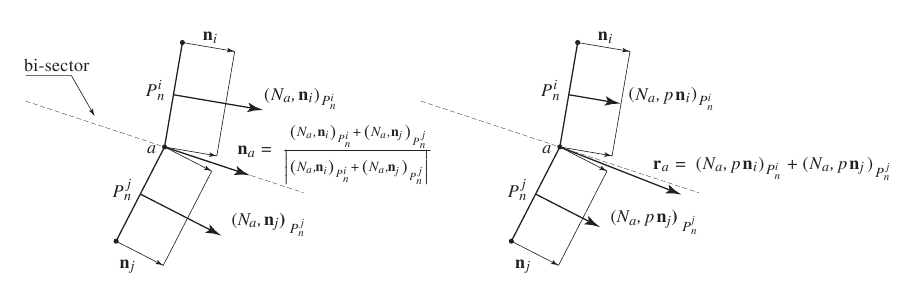
\includegraphics[width=\textwidth]{figures/slip/Behr2004-NormalVsResidual} \\
  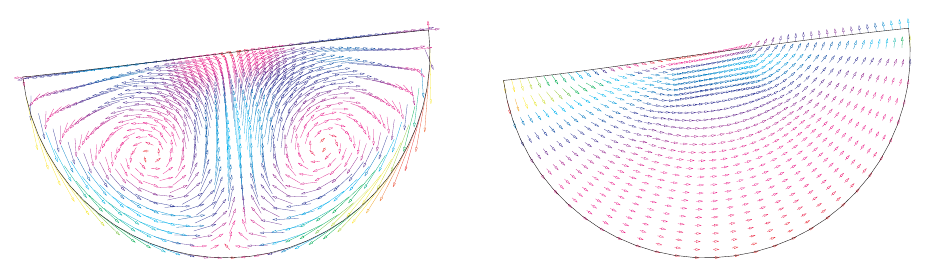
\includegraphics[width=\textwidth]{figures/slip/Behr2004-NavierSloshing} \\
  \footnotesize{(Behr, \emph{On the application of slip boundary condition on curved surfaces}, 2004)}
\end{frame}

\begin{frame}{``No'' boundary condition}
  \begin{itemize}
  \item Integration by parts produces
    \begin{gather*}
      \int_\Gamma \bm v \cdot T \bm\sigma \cdot \bm n, \qquad \bm\sigma = \eta D \bm u - p\bm 1, \qquad T = \bm 1 - \bm n \otimes \bm n
    \end{gather*}
  \item Continuous weak form requires either
    \begin{itemize}
    \item Dirichlet: $\bm u |_{\Gamma} = \bm f \implies \bm v|_\Gamma = 0$
    \item Neumann/Robin: $\bm\sigma\cdot\bm n |_\Gamma = \bm g(\bm u,p)$
    \end{itemize}
  \item Discrete problem allows integration of $\bm\sigma\cdot\bm n$ ``as is''
    \begin{itemize}
    \item Extends validity of equations to include $\Gamma$
    \item \alert{Not valid} for continuum equations
    \item Introduced by Papanastasiou, Malamataris, and Ellwood, 1992 for Navier-Stokes outflow boundaries
    \item Griffiths, {\small \emph{The `no boundary condition' outflow boundary condition}, 1997}
      \begin{itemize}
      \item Proves $L^\infty$ order of accuracy $\bigO((h + 1/\Peclet)^{p+1})$ \\
        for Galerkin finite elements of order $p$ (linear advection-diffusion)
      \item Demonstrates equivalence with collocation at Radau points \\ in outflow element
      \end{itemize}
    \item Used in slip boundary conditions by Behr 2004
    \end{itemize}
  \end{itemize}
\end{frame}


\newcommand{\colorA}[1]{{\color{red} #1}}
\newcommand{\colorB}[1]{{\color{green!60!black} #1}}
\newcommand{\colorC}[1]{{\color{blue} #1}}
\newcommand{\colorD}[1]{{\color{magenta!70!black} #1}}
\newcommand{\colorE}[1]{{\color{cyan!70!black} #1}}
\newcommand{\colorF}[1]{{\color{yellow!60!black} #1}}
\newcommand{\colorG}[1]{{\color{red!50!white} #1}}

\begin{frame}{ALE form}
  After discretization in time ($\alpha \propto 1/\Delta t$) we have a Jacobian
  \begin{equation*}
    \begin{bmatrix}
      \colorA{A_{II}} & \colorA{A_{I\Gamma}}             &                       &                             &                     &   \\
      & \colorB{\alpha M_{\Gamma\Gamma}} &                       & \colorB{- N_{\Gamma\Gamma}} &                       &  \\
      \colorG{G_{II}}      & \colorG{G_{\Gamma I}} & \colorC{B_{II}}       & \colorC{B_{I\Gamma}}        & \colorC{C_{I}^T}    & \colorD{D_I} \\
      \colorG{G_{I\Gamma}} &        \colorG{G_{\Gamma\Gamma}}                          & \colorC{B_{\Gamma I}} & \colorC{B_{\Gamma\Gamma}}   & \colorC{C_{\Gamma}^T} & \colorD{D_\Gamma} \\
      \colorG{G_{Ip}}        &  \colorG{G_{\Gamma p}}                                & \colorC{C_{I}}        & \colorC{C_{\Gamma}}         &                   & \\
      \colorE{\alpha E_I}    & \colorE{\alpha E_\Gamma} & \colorE{F_I} & \colorE{F_\Gamma} & & \colorF{\alpha M_\Theta + J}
    \end{bmatrix}
    \begin{bmatrix}
      x_I \\ x_\Gamma \\ u_I \\ u_\Gamma \\ p \\ \Theta
    \end{bmatrix}
  \end{equation*}
  \begin{itemize}
  \item \colorA{mesh motion equations (Laplace-Beltrami or pseudo-elasticity)}
  \item \colorB{$(\dot{\bm x} - \bm u)\cdot \bm n = \text{accumulution}$}
  \item \colorG{``just'' geometry}
  \item \colorC{Stokes problem}
  \item \colorD{temperature dependence of rheology}
  \item \colorE{convective terms and strain heating in heat transport}
  \item \colorF{thermal advection-diffusion}
  \end{itemize}
\end{frame}


\section{Coupling}
\begin{frame}{Multi-physics coupling in PETSc}
  \begin{columns}
    \begin{column}{0.5\textwidth}
      \tikzstyle{cloud} = [draw, ellipse,fill=red!20, node distance=3cm, minimum height=2em]
      \tikzstyle{block} = [rectangle, draw, fill=blue!20, text width=5em, text centered, rounded corners, minimum height=2em]
      \begin{tikzpicture}
        \node [cloud] (momentum) {Momentum};
        \node [cloud, right of=momentum] (pressure) {Pressure};
        \node<2-> [block, opacity=0.5, fit=(momentum)(pressure), text opacity=0.8] (stokes) {Stokes};
        \node<3-> [cloud, below=2em of momentum] (energy) {Energy};
        \node<3-> [cloud, below=2em of pressure] (geometry) {Geometry};
        \node<4-> [block, opacity=0.4, fit=(stokes)(momentum)(pressure)(energy)(geometry), text opacity=0.8, text height=4em] (ice) {Ice};
        \node<5-> [block, below=2em of ice, minimum width=16em] (bl) {{Boundary \nolinebreak Layer}};
        \node<5-> [block, below=2em of bl, minimum width=16em] (ocean) {Ocean};
        % ]
      \end{tikzpicture}
    \end{column}
    \begin{column}{0.5\textwidth}
      \begin{itemize}
      \item package each ``physics'' independently
      \item solve single-physics and coupled problems
      \item semi-implicit and fully implicit
      \item reuse residual and Jacobian evaluation unmodified
      \item direct solvers, fieldsplit inside multigrid, multigrid inside fieldsplit without recompilation
      \item use the best possible matrix format for each physics \\ (e.g. symmetric block size 3)
      \item matrix-free anywhere
      \item multiple levels of nesting
      \end{itemize}
    \end{column}
  \end{columns}
\end{frame}


\begin{frame}{Outlook}
  \begin{block}{}
    \begin{itemize}
    \item We have textbook multigrid efficiency for hydrostatic equations
    \item Finally a good algebraic interface for tightly-coupled multiphysics
    \item Technical challenges for Stokes
    \item Local conservation is critical, well-balanced slip
    \item Singularities: reentrant corners, transition from frozen \\ \quad 
      to slip bounadry conditions, grounded margins, grounding lines
    \item Stiff geometric coupling terms
    \item IMEX time integration: additive Runge-Kutta
    \end{itemize}    
  \end{block}
  \begin{block}{Tools}
    \begin{itemize}
    \item PETSc\ \url{http://mcs.anl.gov/petsc}
      \begin{itemize}\item ML, Hypre, MUMPS
      \end{itemize}
    \item ITAPS \url{http://itaps.org}
      \begin{itemize}\item MOAB, CGM, Lasso
      \end{itemize}
    \end{itemize}
  \end{block}
\end{frame}

\end{document}
